
% draw of von Neumann machine
\usetikzlibrary{shapes.arrows}
\def\height{1.75cm}
\def\width{2.5cm}
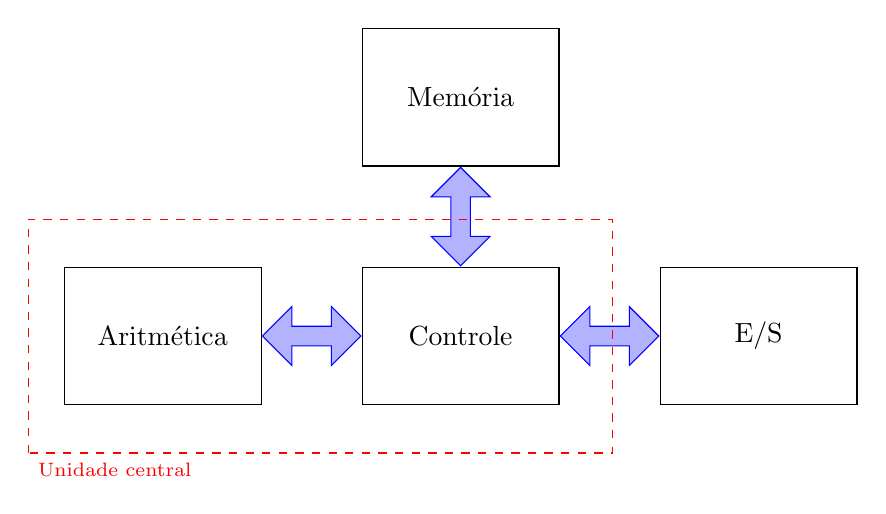
\begin{tikzpicture}[scale=0.9,
  module/.style={anchor=west,draw,rectangle,minimum width=\width,minimum height=\height},
  vdarrow/.style={anchor=west,double arrow,draw=blue,fill=blue!30,minimum height=1.25cm}, % vertical double arrow
  hdarrow/.style={vdarrow,rotate=90} % horizontal double arrow
  ]
  \node[name=a,module] at (0,0) {Aritm\'etica};
  \node[name=ac,vdarrow,shift=(a.east)] {};
  \node[name=c,module,shift=(ac.east)] {Controle};
  \node[name=ces,vdarrow,shift=(c.east)] {};
  \node[name=es,module,shift=(ces.east)] (es) at (2*\height+2*\width,0) {E/S};
  % ATENTION HERE: rotating the double arrow dont change
  % the position names, so east continues being the extremity
  \node[name=ces,hdarrow,shift=(c.north)] {};
  \node[name=mem,module,anchor=south,shift=(ces.east)] {Mem\'oria};
  \draw[dashed,draw=red] (-0.5,-1.65) node[below right]
  {\color{red}{\scriptsize{Unidade central}}} rectangle (7.75,1.65);
\end{tikzpicture}
